\chapter{Statistiken}

    \section{Zahlen}
        \begin{itemize}
            \item Lines of Code: ca. 15000
            \item Commits: ca. 370
        \end{itemize}
        
    \section{Graphen und Statistiken}

		\begin{figure}[ht] 
			\centering
			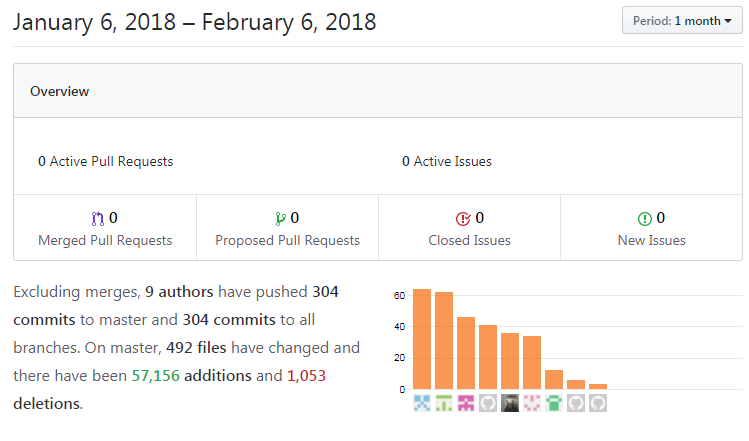
\includegraphics[scale=0.90, trim= 1cm 0 0 0]{pulse.png}
            \caption{GitHub Insights - Pulse}
			\label{fig1}
		\end{figure}

		\begin{figure}[ht] 
			\centering
			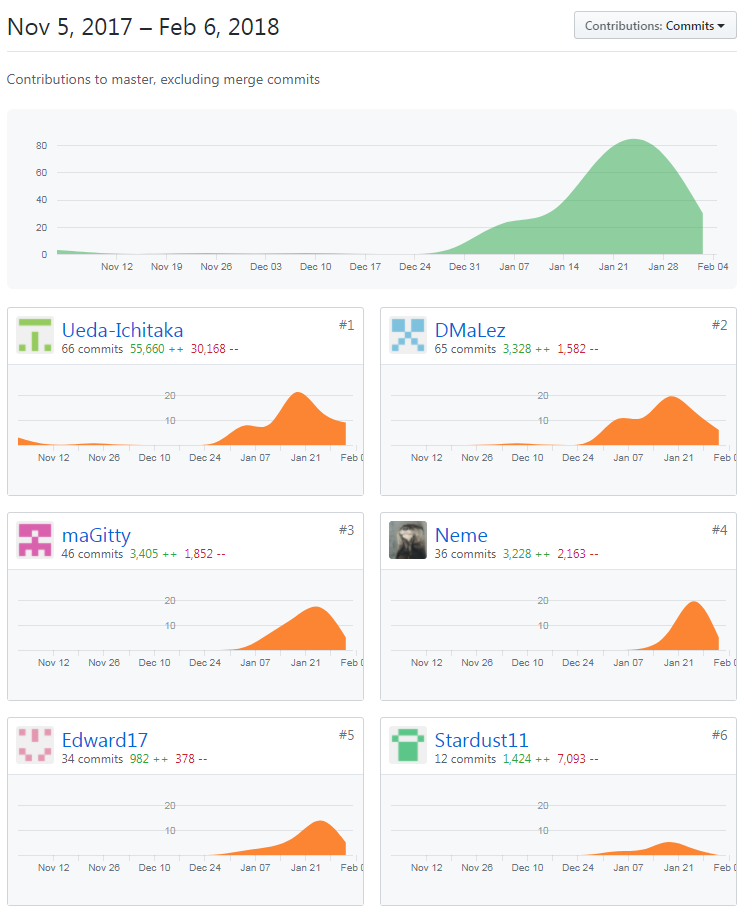
\includegraphics[scale=0.90, trim= 1cm 0 0 0]{contributors.png}
            \caption{GitHub Insights - Contributors}
			\label{fig2}
		\end{figure}

		\begin{figure}[ht] 
    		\centering
			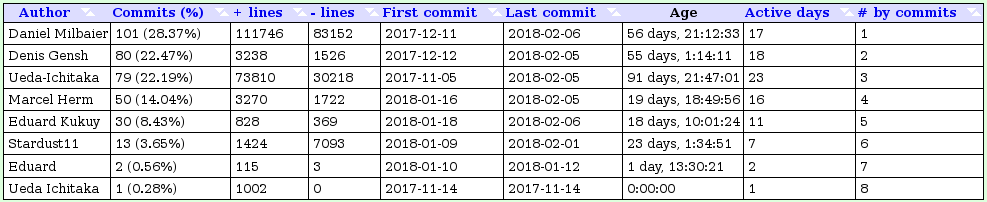
\includegraphics[scale=0.755, trim= 3cm 0 0 0]{authors.png}
            \caption{GitStats - List of Authors}
			\label{fig3}
		\end{figure}
	
		\begin{figure}[ht] 
			\centering
			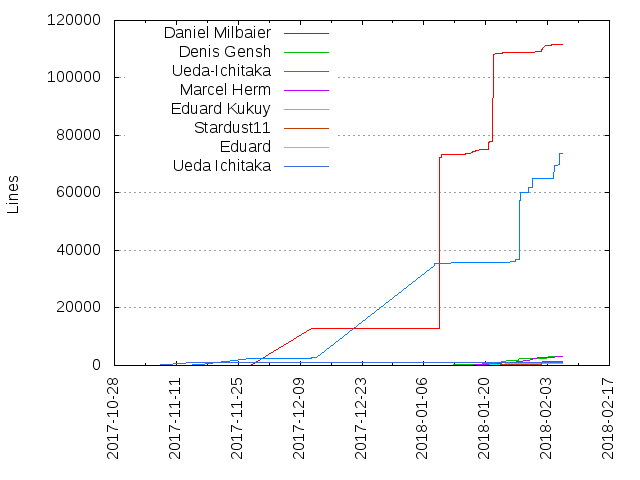
\includegraphics[scale=1.00, trim= 1cm 0 0 0]{lines_of_code_by_author.png}
            \caption{GitStats - Lines of Code per Author}
			\label{fig4}
		\end{figure}

		\begin{figure}[ht] 
			\centering
			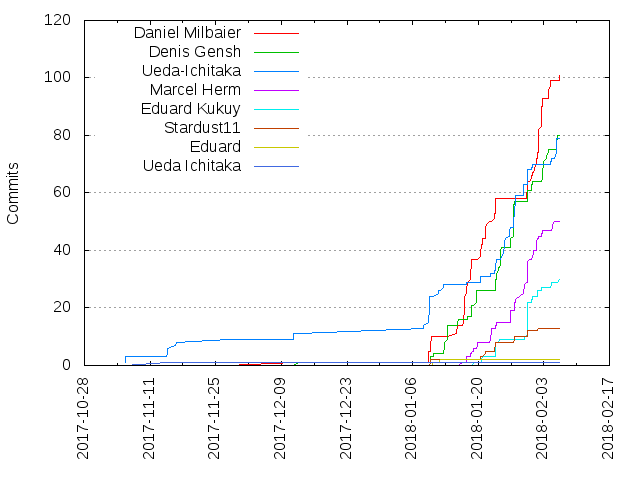
\includegraphics[scale=1.00, trim= 1cm 0 0 0]{commits_by_author.png}
            \caption{GitStats - Commits per Author}	
			\label{fig5}
		\end{figure}
